\documentclass[conference]{IEEEtran}

\usepackage[utf8]{inputenc}
\usepackage[T1]{fontenc}
\usepackage[spanish,es-tabla]{babel}
\usepackage{graphicx}
\usepackage{booktabs}
\usepackage{array}
\usepackage{amsmath}
\usepackage{url}
\usepackage[hidelinks]{hyperref}
\usepackage{cite}

% Correo del autor (cambiar aquí)
\newcommand{\correo}{p306025@uach.mx}

\renewcommand{\arraystretch}{1.1}

\begin{document}

\title{Detección de posible deficiencia de testosterona en hombres adultos con Regresión Logística, SVM, Random Forest y XGBoost}

\author{\IEEEauthorblockN{Jesús Pascual Garay Ordaz}
\IEEEauthorblockA{Matrícula 306025, programa MIC, UACH\\
Materia: Machine Learning. Docente: Dra. Olanda Prieto Ordaz\\
Correo: \correo}}

\maketitle

\begin{abstract}
La deficiencia de testosterona en hombres adultos suele pasar desapercibida ya que solo se confirma con un análisis de sangre, por lo que una herramienta que ayude a decidir a quién pedírselo podría ser útil. Este trabajo plantea el problema como una clasificación binaria (testosterona total menor a 300 ng/dL) con datos de 2514 hombres de la encuesta NHANES 2021 a 2023, de los cuales el 22.2\% tiene la deficiencia, y compara cuatro modelos con un mismo protocolo para que la comparación sea justa. Se evaluaron Regresión Logística, SVM con kernel RBF, Random Forest y XGBoost a partir de 13 variables clínicas, hormonales y de estilo de vida, con una partición estratificada 80/20, un Pipeline que evita la fuga de información, una búsqueda de hiperparámetros con validación cruzada de 5 folds que maximiza el ROC AUC y un umbral de decisión que maximiza la métrica $F_2$. En el conjunto de prueba, de 503 hombres, el SVM obtuvo el mejor ROC AUC (0.901), seguido por XGBoost (0.898), Random Forest (0.892) y Regresión Logística (0.866), aunque la diferencia entre los tres modelos no lineales es menor que la variación entre folds, y todos detectaron cerca del 88\% de los casos con una precisión de 45\% a 55\%. SHBG y estradiol fueron las variables más importantes. Se concluye que los modelos sirven como apoyo para priorizar estudios de laboratorio y no como diagnóstico, y que la comparación con la literatura debe tomarse con cautela por las diferencias de protocolo.
\end{abstract}

\begin{IEEEkeywords}
deficiencia de testosterona, clasificación desbalanceada, SVM, XGBoost, NHANES.
\end{IEEEkeywords}

%==========================================================================
\section{Introducción}

La deficiencia de testosterona, también llamada hipogonadismo bioquímico, es una condición de los hombres adultos que se define con un criterio de laboratorio, ya que la guía de la American Urological Association (AUA) considera razonable un corte de 300 ng/dL para la testosterona total y pide hacer el diagnóstico con dos mediciones tomadas por la mañana en días distintos y con síntomas o signos \cite{mulhall2018}, y la guía de la Endocrine Society coincide en que el diagnóstico requiere síntomas y una testosterona baja de forma consistente \cite{bhasin2018}. Se asocia con obesidad, diabetes e hipertensión, y entre sus consecuencias están la pérdida de masa muscular, la osteoporosis y los problemas metabólicos, lo que le da relevancia clínica.

El problema es que la condición solo se detecta cuando alguien pide el análisis, por lo que muchos casos pasan desapercibidos, y una herramienta que use datos fáciles de obtener, como las medidas corporales y los antecedentes, podría ayudar a decidir a quién conviene pedírselo. Las soluciones computacionales que existen son de dos tipos, los índices sencillos de tamizaje basados en medidas antropométricas y metabólicas \cite{zhang2025, guo2025, xu2024} y los modelos de Machine Learning (ML) entrenados con encuestas poblacionales o con cohortes clínicas \cite{yu2025, novaes2021, kivrak2024}, y mientras los primeros son fáciles de calcular pero usan pocas variables, los segundos pueden combinar muchas.

El objetivo de este trabajo es construir y comparar cuatro modelos de clasificación, Regresión Logística, SVM, Random Forest y XGBoost, para identificar a hombres adultos con deficiencia de testosterona a partir de 13 variables de la encuesta NHANES 2021 a 2023 \cite{cdc_nhanes}, y ponerlos a disposición mediante una interfaz web. El alcance es el de un proyecto académico, ya que se usa una sola base de datos, una sola partición y la definición bioquímica de la deficiencia con una medición por persona, lo que lleva a plantear los modelos como apoyo para priorizar estudios de laboratorio y no como herramienta diagnóstica. En lo que sigue se revisan los trabajos relacionados (sección~\ref{sec:antecedentes}), se describe la metodología (sección~\ref{sec:metodologia}), se presentan y discuten los resultados (sección~\ref{sec:resultados}) y se concluye (sección~\ref{sec:conclusiones}).

%==========================================================================
\section{Antecedentes y trabajos relacionados}
\label{sec:antecedentes}

Los trabajos más cercanos al mío usan NHANES y el mismo criterio de 300 ng/dL, aunque con otros ciclos de la encuesta, otras variables y otros objetivos. Yu et al. \cite{yu2025} usan NHANES 2011 a 2014 (2628 hombres, 25.76\% con deficiencia) para probar si el índice de calidad muscular mejora la predicción, con 18 predictoras, una partición 80/20 y validación cruzada de 5 folds, y comparan seis modelos de ML, de los cuales el mejor fue LightGBM con un AUC de 0.746 mientras que el SVM obtuvo 0.713. Zhang et al. \cite{zhang2025} analizan 1514 hombres de NHANES 2013 a 2016 y comparan nueve índices sencillos de tamizaje, entre los que el mejor, el producto del índice triglicéridos-glucosa por la relación cintura-estatura (TyG-WHtR), alcanzó un AUC de 0.776. Guo et al. \cite{guo2025} evalúan 15 índices de obesidad y lípidos con 3540 hombres de NHANES 2011 a 2016 y de nuevo el TyG-WHtR fue el mejor con un AUC de 0.762, y Xu y Li \cite{xu2024} encuentran con 5012 hombres de NHANES 2013 a 2020 que el índice cardiometabólico alcanza un AUC de 0.724, con una sensibilidad de 60.1\% y una especificidad de 71.3\%. Por último, Goulian et al. \cite{goulian2026} usan los ciclos 2011 a 2016 y 2021 a 2023 (10357 participantes) con un enfoque explicativo basado en regresión logística, y reportan que la prevalencia bajó de 25.7\% a 20.3\% en el último ciclo y que la obesidad se asocia con la deficiencia (razón de momios ajustada de 2.69), sin dar un AUC.

Otros dos trabajos tratan el mismo problema con datos que no son de NHANES. Novaes et al. \cite{novaes2021} comparan 10 clasificadores base y tres ensambles con una cohorte hospitalaria de Brasil de 3397 pacientes, y encuentran que XGBoost fue el mejor clasificador base y que el ensamble por promedio ponderado tuvo el mejor desempeño general, y Kivrak et al. \cite{kivrak2024} estudian el efecto de SMOTE con 1886 pacientes con diabetes tipo 2 y solo cinco predictoras, con una partición 70/30 y validación cruzada estratificada de 10 folds, a lo que con SMOTE la sensibilidad de XGBoost llegó a 0.52 mientras que la de la regresión logística fue de 0.31.

Estos trabajos muestran dos cosas que guían el proyecto, que los modelos basados en árboles y los ensambles suelen ser competitivos, y que con clases desbalanceadas la sensibilidad exige un tratamiento específico. También tienen limitaciones que condicionan la comparación, ya que cambian la población, las variables, las particiones y las métricas, y en el caso de Yu et al. \cite{yu2025} los seis modelos reportan un recall de 1.000, lo que impide comparar el recall y deja al AUC como la única métrica comparable. Lo que distingue a esta evaluación es que incluye entre las predictoras a SHBG, estradiol, LH y FSH, que pertenecen al mismo eje hormonal que la testosterona y que no forman parte de los índices de los otros trabajos, que elige el umbral de decisión con predicciones fuera de muestra y no con el conjunto de prueba, que separa la validación del resultado final en una prueba usada una sola vez, y que usa el ciclo más reciente de la encuesta (2021 a 2023).

%==========================================================================
\section{Metodología}
\label{sec:metodologia}

La Figura~\ref{fig:metodologia} resume el flujo completo, desde la construcción de la base hasta la evaluación final.

\begin{figure*}[!t]
\centering
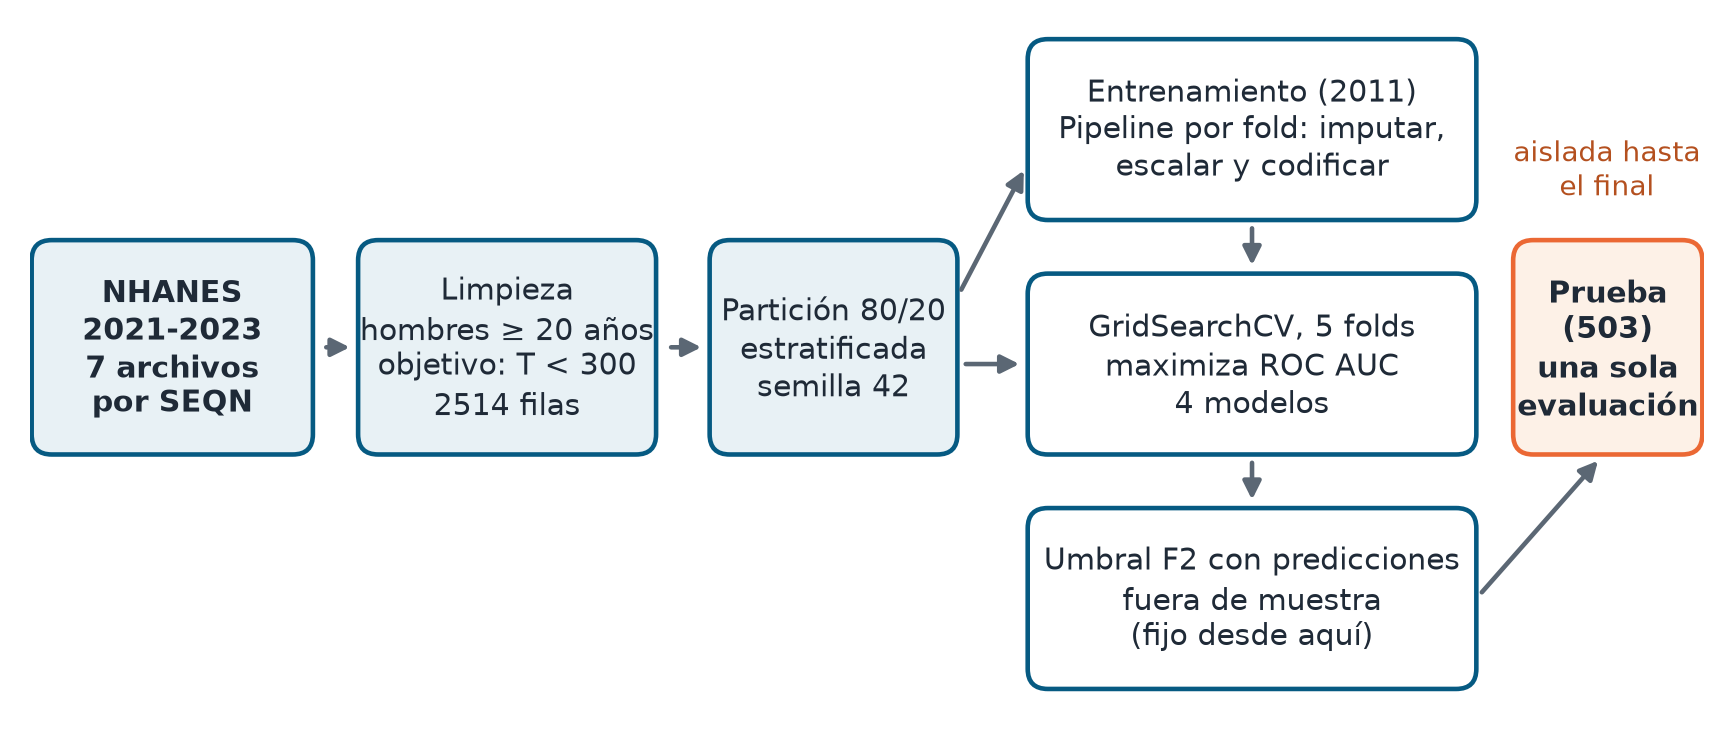
\includegraphics[width=0.82\textwidth]{figuras/diagrama_metodologia.png}
\caption{Diagrama general de la metodología. El conjunto de prueba se aísla en la partición y no se usa para ajustar, seleccionar hiperparámetros ni elegir umbrales.}
\label{fig:metodologia}
\end{figure*}

\subsection{Descripción de la base de datos}

Los datos provienen de la encuesta NHANES (National Health and Nutrition Examination Survey) del National Center for Health Statistics del CDC, ciclo 2021 a 2023 \cite{cdc_nhanes}, cuyo propósito original es evaluar el estado de salud y nutrición de la población de Estados Unidos mediante entrevistas y exámenes físicos y de laboratorio. Se unieron siete archivos por el identificador del participante (\texttt{SEQN}) partiendo de los datos demográficos: demografía (DEMO\_L), panel de hormonas esteroides sexuales (TST\_L), medidas corporales (BMX\_L), diabetes (DIQ\_L), presión arterial (BPQ\_L), alcohol (ALQ\_L) y tabaco (SMQ\_L). Después se conservaron solo los hombres de 20 años o más con la testosterona total medida, se eliminaron los duplicados y toda fila con más de 30\% de datos faltantes entre las predictoras, lo que dejó \textbf{2514 hombres}, y el consumo de alcohol se fijó en cero cuando el participante nunca tomó o no tomó en los últimos 12 meses, ya que en esos casos NHANES no hace la pregunta y el valor queda en blanco aunque el consumo real es cero.

La variable objetivo es \texttt{deficiencia\_testosterona}, que vale 1 cuando la testosterona total es menor a 300 ng/dL y 0 en caso contrario \cite{mulhall2018}, lo que da una clasificación binaria con 1955 hombres normales (77.8\%) y 559 con deficiencia (22.2\%), es decir, con clases desbalanceadas. Se usan 13 variables predictoras, 8 numéricas y 5 categóricas (Tabla~\ref{tab:variables}), y se excluyeron el identificador, que no tiene significado clínico, y la testosterona total, ya que con ella se calcula el objetivo y dejarla permitiría acertar casi perfecto sin aprender nada útil, lo que sería fuga de información. Como limitaciones del conjunto, la deficiencia se define con una sola medición por participante y no con el diagnóstico clínico completo, algunas variables son autorreportadas, es un estudio transversal de Estados Unidos y no se usaron los pesos muestrales del diseño complejo de la encuesta, por lo que los resultados no representan a la población.

\begin{table}[t]
\centering
\footnotesize
\caption{Variables predictoras.}
\label{tab:variables}
\begin{tabular}{l l p{4.6cm}}
\toprule
Variable (código) & Tipo & Descripción \\
\midrule
edad (RIDAGEYR) & Num. & Edad en años (20 a 80) \\
imc (BMXBMI) & Num. & Índice de masa corporal (kg/m$^2$) \\
cintura (BMXWAIST) & Num. & Circunferencia de cintura (cm) \\
shbg (LBXSHBG) & Num. & Globulina fijadora de hormonas sexuales (nmol/L) \\
estradiol (LBXEST) & Num. & Estradiol (pg/mL) \\
lh (LBXLUH) & Num. & Hormona luteinizante (mIU/mL) \\
fsh (LBXFSH) & Num. & Hormona folículo estimulante (mIU/mL) \\
tragos\_por\_dia (ALQ130) & Num. & Tragos de alcohol por día, últimos 12 meses \\
diabetes (DIQ010) & Cat. & Sí, No o Prediabetes \\
hipertension (BPQ020) & Cat. & Diagnóstico de hipertensión \\
fumador (SMQ020) & Cat. & Al menos 100 cigarrillos en la vida \\
raza\_etnia (RIDRETH3) & Cat. & Seis categorías \\
escolaridad (DMDEDUC2) & Cat. & Cinco niveles \\
\bottomrule
\end{tabular}
\end{table}

\subsection{Análisis exploratorio y preprocesamiento}

El análisis exploratorio se hizo solo sobre el conjunto de entrenamiento, y lo primero que se vio es que los faltantes se concentran en el consumo de alcohol (12.4\%), seguido de la cintura (3.7\%), el IMC (1.2\%) y el estradiol (0.5\%), y que además hay respuestas de «rehuso» o «no sabe» que NHANES guarda como números (7, 9, 777 y 999) y que en realidad también son faltantes, por lo que se convierten en valores vacíos y se imputan dentro del Pipeline con la mediana en las numéricas y la moda en las categóricas, lo que además permite que la interfaz deje una variable vacía. Las escalas de las variables son muy distintas, por ejemplo la edad va de 20 a 80 mientras que la SHBG llega a 232.6, así que las numéricas se escalan con \texttt{StandardScaler}, algo necesario para la Regresión Logística y el SVM que son sensibles a la escala, y las categóricas se codifican con \texttt{OneHotEncoder}. Las hormonas tienen distribuciones cargadas a la derecha con valores extremos, y con el criterio del rango intercuartílico (IQR) se identificó un 9.6\% de valores atípicos en la FSH y un 6.8\% en la LH, que no se eliminaron porque son valores fisiológicamente posibles y porque los modelos de árboles son robustos a ellos, mientras que en los modelos sensibles el escalamiento y la regularización amortiguan su efecto.

Las variables más relacionadas con el objetivo (Figura~\ref{fig:correlaciones}) son la cintura (0.31) y el IMC (0.31) en sentido positivo, y la SHBG ($-$0.29) y el estradiol ($-$0.24) en sentido negativo, es decir, que a más obesidad y menor SHBG y estradiol, mayor frecuencia de deficiencia. Entre las categóricas, la deficiencia es más frecuente en quienes tienen diabetes (36.3\% contra 19.2\%) y en quienes tienen hipertensión (27.1\% contra 19.1\%), y también hay pares de predictoras muy correlacionadas entre sí, el IMC con la cintura (0.92) y la LH con la FSH (0.84). No se hizo selección ni reducción de características y se conservaron las 13 variables, ya que son pocas, tienen sentido clínico y la regularización de la Regresión Logística y la forma en que los árboles dividen reducen el efecto de la colinealidad.

\begin{figure}[t]
\centering
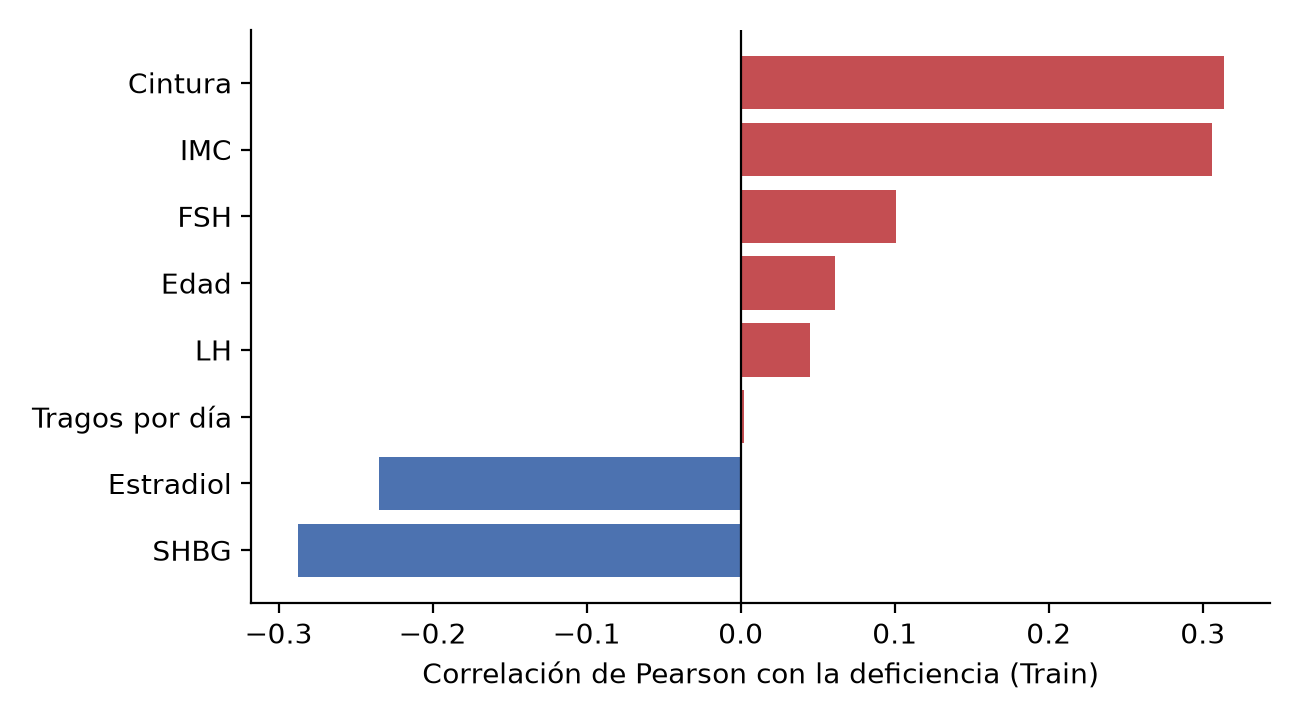
\includegraphics[width=0.92\columnwidth]{figuras/correlaciones.png}
\caption{Correlación de Pearson de cada variable numérica con la deficiencia de testosterona en el conjunto de entrenamiento.}
\label{fig:correlaciones}
\end{figure}

\textbf{Desbalance de clases.} Como la clase positiva es solo el 22.2\%, un modelo que siempre dijera «normal» acertaría el 77.8\% sin detectar a nadie, por lo que la exactitud se usó solo como referencia y el desbalance se atacó de tres formas, con el peso de clases (\texttt{class\_weight=balanced} y \texttt{scale\_pos\_weight} en XGBoost) como hiperparámetro a explorar, con métricas que no dependen de la proporción (ROC AUC y precisión-recall) y con la elección del umbral de decisión. No se usó SMOTE ya que generaría observaciones sintéticas de variables numéricas mezcladas con categóricas y faltantes, y porque el umbral y el peso de clases logran un efecto parecido sin alterar los datos.

\textbf{Fuga de información.} La partición se hace antes de cualquier ajuste, las reglas fijas (convertir códigos de rehuso en faltantes y dar nombre a los códigos categóricos) no aprenden nada de los datos, y todo lo que sí aprende (medianas, modas, medias, desviaciones y categorías) vive dentro de un \texttt{Pipeline} de scikit-learn \cite{pedregosa2011, sklearn_compose} que se ajusta solo con los datos de entrenamiento de cada fold. Los hiperparámetros se eligen con validación cruzada y los umbrales con predicciones fuera de muestra, ambos sobre el conjunto de entrenamiento, por lo que el conjunto de prueba solo se usa una vez al final.

\subsection{Modelos de Machine Learning}

Se compararon cuatro modelos de familias distintas, y de los cuatro se obtiene la probabilidad de pertenecer a la clase «deficiencia».

\textbf{Regresión Logística.} Modela la probabilidad como
\begin{equation}
P(y=1\mid \mathbf{x})=\sigma(\mathbf{w}^{\top}\mathbf{x}+b)=\frac{1}{1+e^{-(\mathbf{w}^{\top}\mathbf{x}+b)}},
\end{equation}
donde $\mathbf{x}$ es el vector de las 13 variables, $\mathbf{w}$ los coeficientes y $b$ el sesgo. Se eligió porque es el modelo más sencillo de interpretar y sirve como punto de partida de comparación \cite{garay_f1}, y se exploró la regularización L1 y L2 y el parámetro $C$, que a mayor valor da menos regularización.

\textbf{SVM con kernel RBF.} Busca la frontera de máximo margen entre las clases y, con el kernel
\begin{equation}
K(\mathbf{x},\mathbf{x}')=\exp\left(-\gamma\lVert \mathbf{x}-\mathbf{x}'\rVert^2\right),
\end{equation}
permite fronteras no lineales \cite{cortes1995, sklearn_svm}. Sus hiperparámetros son $C$, que controla cuánto se castigan los errores y las violaciones del margen, y $\gamma$, que define qué tan lejos llega la influencia de cada punto. Se incluyó porque maneja bien pocas variables con relaciones no lineales \cite{garay_f2}, y como no entrega probabilidades por sí solo se calibró con una función sigmoide (\texttt{CalibratedClassifierCV}).

\textbf{Random Forest.} Es un conjunto de árboles de decisión entrenados con muestras aleatorias de los datos y de las variables, cuya predicción es el promedio de los árboles, lo que reduce la varianza de los árboles individuales \cite{breiman2001}. Se eligió por su robustez a valores atípicos y a variables correlacionadas, y porque captura interacciones sin suponer la forma de la relación.

\textbf{XGBoost.} Es una implementación de \emph{gradient boosting} en la que los árboles se construyen en secuencia y cada uno corrige los errores del anterior \cite{chen2016, xgboost_docs}. Se eligió porque suele ser de los mejores modelos en datos tabulares y porque fue el mejor clasificador base en Novaes et al. \cite{novaes2021} y en Kivrak et al. \cite{kivrak2024}, y sus hiperparámetros principales son el número de árboles, la tasa de aprendizaje, la profundidad máxima y el muestreo de filas y columnas.

\subsection{Configuración experimental}

Los datos se dividieron en 80\% para entrenamiento (2011 hombres) y 20\% para prueba (503 hombres) de forma estratificada con semilla 42, de modo que ambos conservan el 22.2\% de casos positivos. El proceso tiene tres etapas separadas, el entrenamiento y la optimización de hiperparámetros con validación cruzada estratificada de 5 folds sobre el conjunto de entrenamiento, la selección del umbral con las predicciones fuera de muestra de esa misma validación, y la evaluación final de los modelos ajustados con todo el entrenamiento en el conjunto de prueba, que se usa una sola vez.

Como modelos base se usaron los de scikit-learn con parámetros por defecto: Regresión Logística con \texttt{max\_iter}=1000, SVM con kernel RBF, Random Forest con 300 árboles y XGBoost con 300 árboles, sin compensar el desbalance. La optimización usa \texttt{GridSearchCV} \cite{sklearn_cv} con el ROC AUC como criterio, una métrica que mide qué tan bien el modelo ordena a los hombres con deficiencia por encima de los normales sin depender de un umbral, y las rejillas y la mejor combinación de cada modelo se muestran en la Tabla~\ref{tab:rejillas}.

\begin{table*}[!t]
\centering
\footnotesize
\caption{Búsqueda de hiperparámetros y mejor combinación de cada modelo (ROC AUC en validación cruzada de 5 folds).}
\label{tab:rejillas}
\begin{tabular}{l p{7.2cm} c p{5.6cm}}
\toprule
Modelo & Hiperparámetros explorados & Comb. & Mejor combinación \\
\midrule
Regresión Logística & $C\in\{0.01,0.1,1,10,100\}$, regularización L1 o L2, \texttt{class\_weight} & 20 & $C$=0.1, L1, \texttt{balanced} \\
SVM (RBF) & $C\in\{0.01,\ldots,100\}$, $\gamma\in\{\texttt{scale},0.001,\ldots,10\}$, \texttt{class\_weight} & 60 & $C$=10, $\gamma$=0.01, \texttt{balanced} \\
Random Forest (300 árboles) & \texttt{max\_depth}$\in\{$sin límite, 5, 10$\}$, \texttt{min\_samples\_leaf}$\in\{1,3,5,10\}$, \texttt{max\_features}$\in\{$sqrt, 0.5$\}$, \texttt{class\_weight} & 48 & sin límite, \texttt{min\_samples\_leaf}=3, \texttt{max\_features}=0.5, \texttt{balanced} \\
XGBoost & \texttt{n\_estimators}$\in\{100,300\}$, \texttt{learning\_rate}$\in\{0.03,0.1\}$, \texttt{max\_depth}$\in\{2,3,5\}$, \texttt{subsample} y \texttt{colsample\_bytree}$\in\{0.7,1\}$, \texttt{scale\_pos\_weight}$\in\{1, \approx3.5\}$ & 96 & 300 árboles, \texttt{learning\_rate}=0.03, \texttt{max\_depth}=2, \texttt{subsample}=0.7, \texttt{colsample\_bytree}=0.7, sin ponderar \\
\bottomrule
\end{tabular}
\end{table*}

Con el umbral estándar de 0.5 los modelos detectan solo a una parte de los casos, por lo que para cada modelo se eligió el umbral que maximiza la métrica $F_2$ con las probabilidades fuera de muestra del conjunto de entrenamiento, y que queda fijo desde ese momento. Con TP, FP y FN los verdaderos positivos, falsos positivos y falsos negativos, las métricas son
\begin{equation}
\text{Precisión}=\frac{TP}{TP+FP},\quad \text{Recall}=\frac{TP}{TP+FN},
\end{equation}
\begin{equation}
F_\beta=\frac{(1+\beta^2)\,\text{Precisión}\cdot\text{Recall}}{\beta^2\,\text{Precisión}+\text{Recall}},\quad \beta=2\ (F_2).
\end{equation}
Se prefirió $F_2$ porque en este problema dejar escapar un caso (falso negativo) cuesta más que pedir un análisis de sangre de más (falso positivo), y se reportan además la exactitud, el $F_1$, el ROC AUC y el promedio de precisión (AP) de la curva precisión-recall, que es más informativo que el ROC AUC cuando la clase positiva es minoritaria.

Todo se implementó en Python 3.12 con scikit-learn 1.9.1 \cite{pedregosa2011}, XGBoost 3.4.1, pandas 3.1.0, NumPy 2.5.4, Matplotlib 3.11.2 y Streamlit 1.66.1 \cite{streamlit_docs}, con semilla 42 en todos los procesos aleatorios. El código, los modelos guardados, las versiones exactas y las instrucciones para reproducir los experimentos están en el repositorio del proyecto\footnote{\url{https://github.com/paskcual/deteccion-testosterona-ml}}, y la interfaz en Streamlit con los tres modelos de mejor ROC AUC en validación cruzada está desplegada en \url{https://deteccion-testosterona-ml.streamlit.app/}.

\subsection{Interfaz de usuario}

Los modelos entrenados con el conjunto de entrenamiento se guardaron con \texttt{joblib}, junto con un archivo de metadatos con los umbrales, las métricas y el rango de cada variable, y se usan desde una aplicación en Streamlit. La interfaz pide las 13 variables, con rangos y valores iniciales tomados de los datos de entrenamiento, y permite dejar vacíos el IMC, la cintura, el estradiol y los tragos por día, que son las variables con faltantes, por lo que el Pipeline los reemplaza por la mediana. La versión desplegada usa los tres modelos de mejor ROC AUC en validación cruzada (XGBoost, Random Forest y SVM), y la captura de la Figura~\ref{fig:interfaz} es de una versión previa que mostraba los cuatro. Al presionar el botón de predicción muestra, para cada modelo, la probabilidad de deficiencia, su umbral y si marca posible deficiencia, junto con un resumen de cuántos modelos coinciden (Figura~\ref{fig:interfaz}), y advierte que es un proyecto académico y no un dispositivo médico. Como ilustración, con un hombre de 55 años con IMC de 33.0, SHBG de 25.0 nmol/L, estradiol de 28.0 pg/mL, diabetes, hipertensión y la cintura vacía, los cuatro modelos superan su umbral (Regresión Logística 0.619, SVM 0.372, Random Forest 0.754 y XGBoost 0.419), lo que es una señal más confiable que cuando solo uno de ellos marca posible deficiencia.

\begin{figure}[t]
\centering
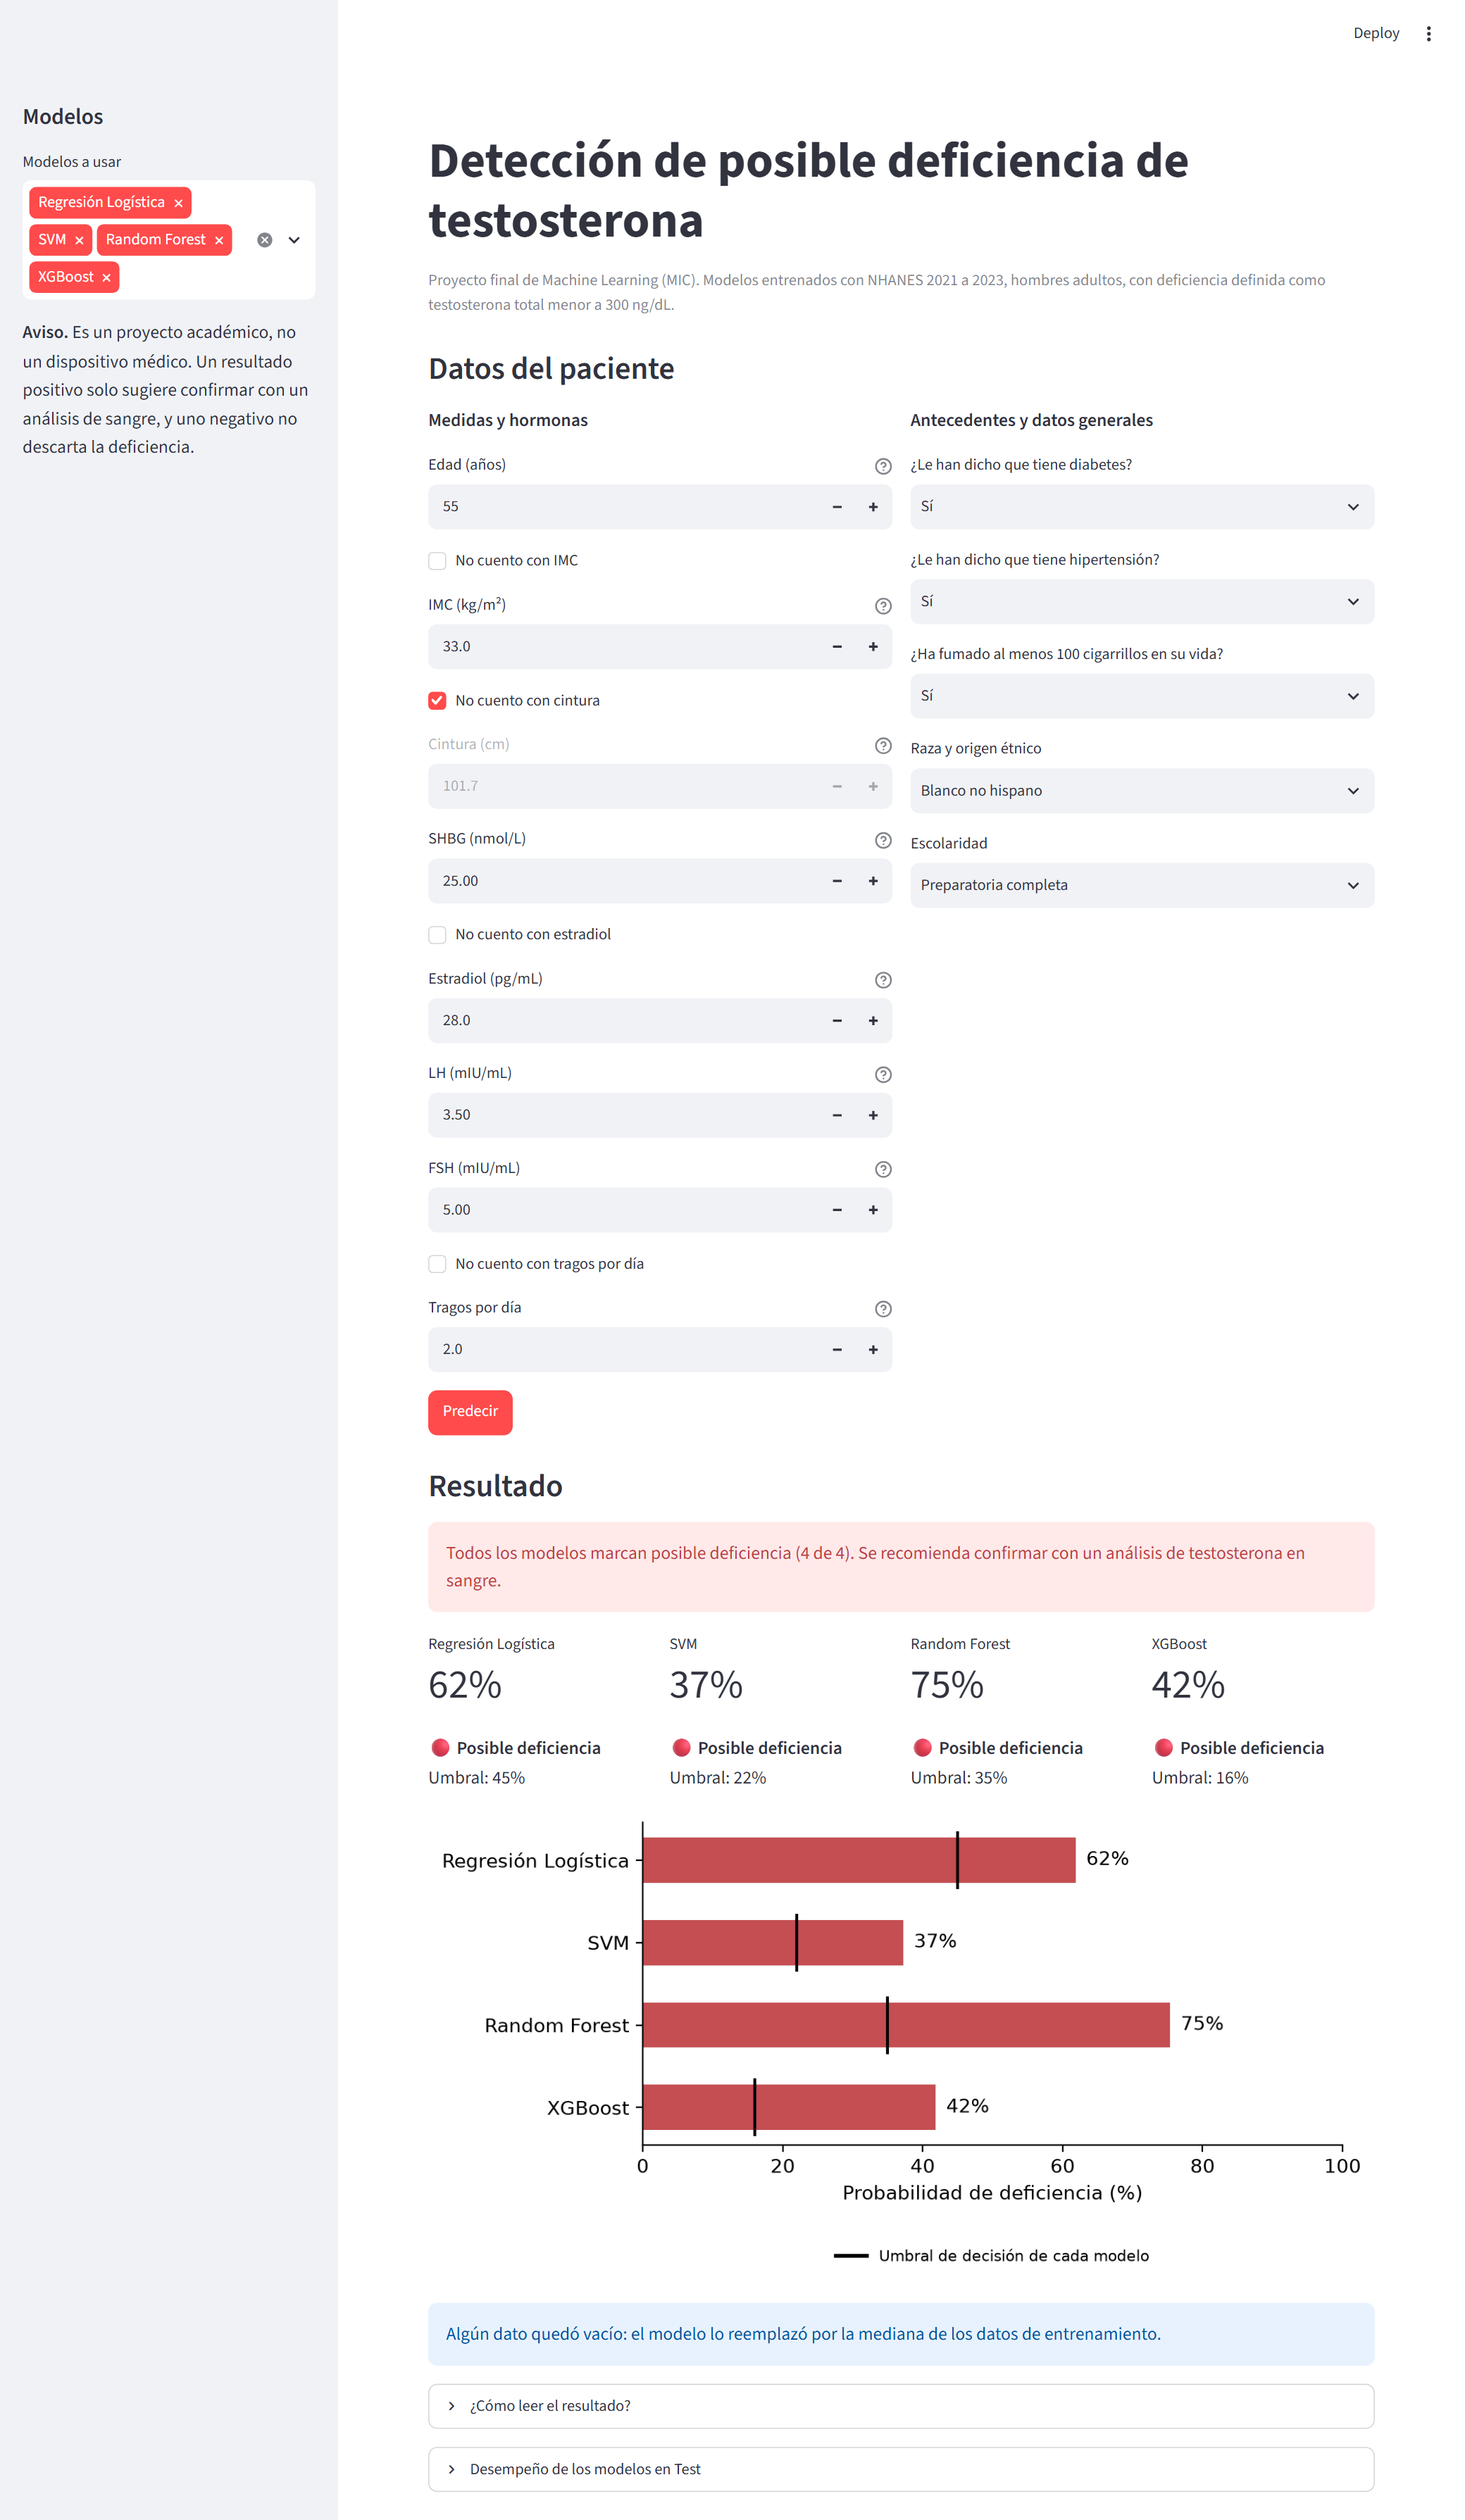
\includegraphics[width=0.62\columnwidth]{figuras/interfaz_resultado.png}
\caption{Interfaz en Streamlit con el caso de ejemplo: datos capturados (con la cintura vacía) y resultado de los modelos.}
\label{fig:interfaz}
\end{figure}

%==========================================================================
\section{Resultados y discusión}
\label{sec:resultados}

\subsection{Resultados de los modelos base}

Con los parámetros por defecto (Tabla~\ref{tab:defecto}) los cuatro modelos quedan en un ROC AUC de 0.864 a 0.890 en validación cruzada, con Random Forest como el mejor, y todos comparten el mismo problema, ya que el recall se queda entre 0.48 y 0.56, es decir, detectan a solo la mitad de los hombres con deficiencia porque ninguno compensa el desbalance de clases. Random Forest y XGBoost además llegan a un ROC AUC de 1.000 en los folds de entrenamiento, lo que muestra que memorizan los datos y necesitan regularización, mientras que la Regresión Logística, con 0.876, apenas se distingue entre entrenamiento y validación.

\begin{table}[t]
\centering
\footnotesize
\setlength{\tabcolsep}{3pt}
\caption{Modelos base con parámetros por defecto: promedio de la validación cruzada de 5 folds con umbral 0.5.}
\label{tab:defecto}
\begin{tabular}{l c c c c c c}
\toprule
Modelo & Exact. & Prec. & Recall & F1 & AUC val. & AUC entr. \\
\midrule
Reg. Logística & 0.841 & 0.696 & 0.508 & 0.584 & 0.866 & 0.876 \\
SVM (RBF) & 0.841 & 0.716 & 0.481 & 0.573 & 0.877 & 0.932 \\
Random Forest & 0.854 & 0.756 & 0.510 & 0.608 & 0.890 & 1.000 \\
XGBoost & 0.833 & 0.645 & 0.562 & 0.600 & 0.864 & 1.000 \\
\bottomrule
\end{tabular}
\end{table}

\subsection{Resultados de los modelos optimizados}

La optimización (Tabla~\ref{tab:optimizados}) ayudó poco a la Regresión Logística, al SVM y al Random Forest (de 0.003 a 0.007 de ROC AUC), pero mucho a XGBoost, que subió de 0.864 a 0.896 y bajó su ROC AUC de entrenamiento de 1.000 a 0.934, ya que eligió árboles de profundidad 2 con una tasa de aprendizaje de 0.03 y muestreo de filas y columnas, lo que sugiere que la relación entre las variables y la deficiencia es suave y con pocas interacciones. Los tres mejores modelos quedan casi empatados, porque sus diferencias (0.896, 0.894 y 0.884) son menores o parecidas a la desviación entre folds, y como las mejoras de 0.003 a 0.007 también lo son, no se consideran mejoras concluyentes.

\begin{table}[t]
\centering
\footnotesize
\setlength{\tabcolsep}{3pt}
\caption{Modelos optimizados. ROC AUC de validación cruzada (media y desviación entre folds) y desempeño en el conjunto de prueba con el umbral elegido (503 hombres, 112 con deficiencia).}
\label{tab:optimizados}
\begin{tabular}{l c c c c c c c}
\toprule
Modelo & AUC val. & Desv. & Umbral & Prec. & Recall & F1 & AUC prueba \\
\midrule
Reg. Logística & 0.868 & 0.019 & 0.45 & 0.454 & 0.875 & 0.598 & 0.866 \\
SVM (RBF) & 0.884 & 0.022 & 0.22 & 0.553 & 0.884 & 0.680 & 0.901 \\
Random Forest & 0.894 & 0.008 & 0.35 & 0.551 & 0.875 & 0.676 & 0.892 \\
XGBoost & 0.896 & 0.014 & 0.16 & 0.505 & 0.884 & 0.643 & 0.898 \\
\bottomrule
\end{tabular}
\end{table}

\begin{figure}[t]
\centering
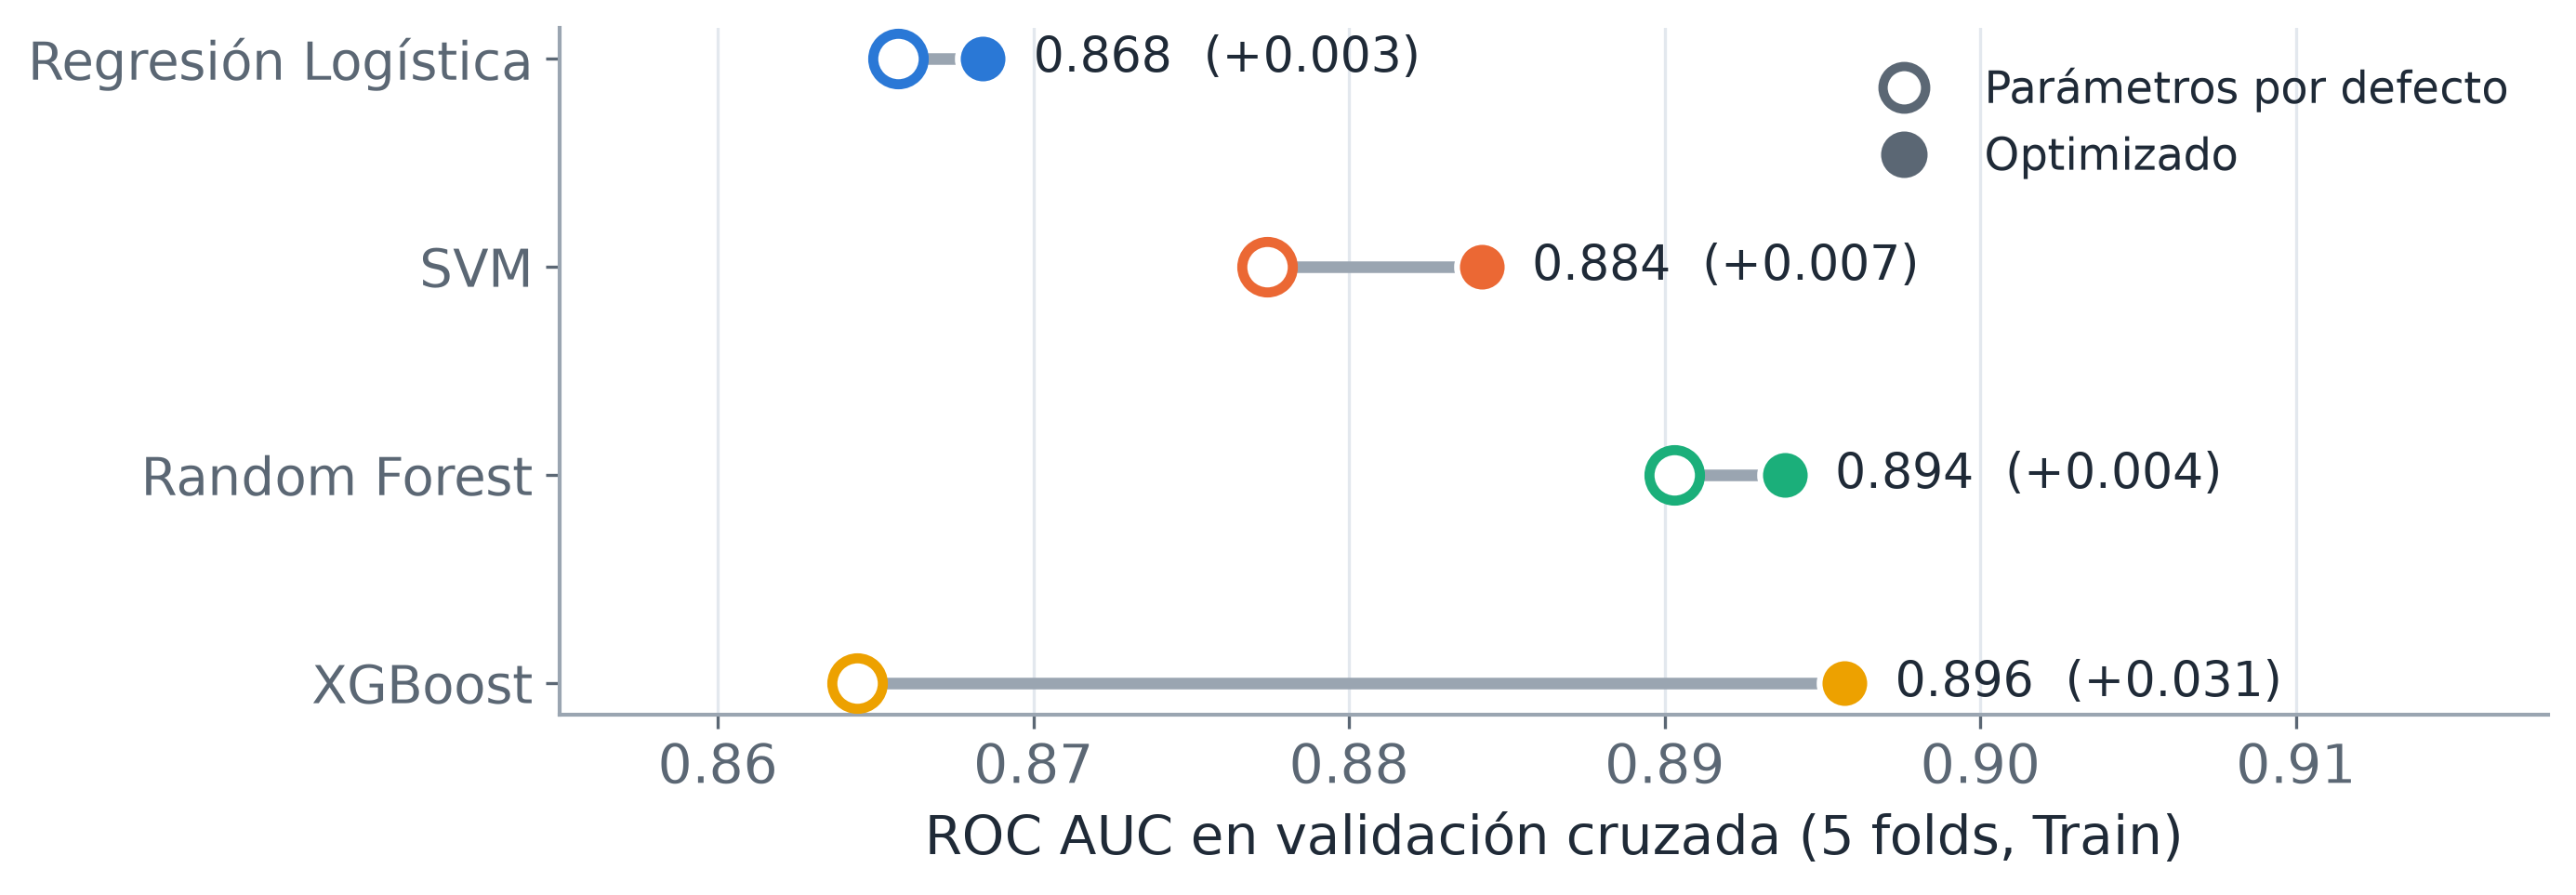
\includegraphics[width=\columnwidth]{figuras/auc_base_vs_optimizado.png}
\caption{ROC AUC en validación cruzada de cada modelo con parámetros por defecto (círculo vacío) y optimizado (círculo lleno). El eje no empieza en cero para que se aprecie la diferencia, que fue de 0.003 a 0.007 salvo en XGBoost (0.031).}
\label{fig:base_opt}
\end{figure}

El umbral que maximiza $F_2$ es distinto en cada modelo, 0.45 en la Regresión Logística, 0.35 en Random Forest, 0.22 en SVM y 0.16 en XGBoost, lo que no significa que unos sean mejores que otros sino que cada uno reparte sus probabilidades de forma diferente. Con esos umbrales los cuatro quedan en un recall de 0.85 a 0.88 en las predicciones fuera de muestra del entrenamiento, y lo que cambia es el costo en falsas alarmas, que va de 357 en el SVM a 437 en la Regresión Logística. La Figura~\ref{fig:umbrales} muestra cómo cambian la precisión, el recall y $F_2$ al mover el umbral, y la Tabla~\ref{tab:oof} resume el resultado de cada modelo con el umbral elegido sobre esas predicciones fuera de muestra, donde se ve que el recall de 0.85 a 0.88 se logra a costa de una precisión de 0.47 a 0.52.

\begin{table}[t]
\centering
\footnotesize
\setlength{\tabcolsep}{3pt}
\caption{Predicciones fuera de muestra sobre el conjunto de entrenamiento (2011 hombres, 447 con deficiencia) con el umbral elegido.}
\label{tab:oof}
\begin{tabular}{l c c c c c c c c}
\toprule
Modelo & Umbral & Prec. & Recall & F1 & AUC & FP & FN & TP \\
\midrule
Reg. Logística & 0.45 & 0.472 & 0.872 & 0.612 & 0.868 & 437 & 57 & 390 \\
SVM (RBF) & 0.22 & 0.516 & 0.852 & 0.643 & 0.883 & 357 & 66 & 381 \\
Random Forest & 0.35 & 0.511 & 0.868 & 0.643 & 0.892 & 371 & 59 & 388 \\
XGBoost & 0.16 & 0.496 & 0.881 & 0.634 & 0.895 & 401 & 53 & 394 \\
\bottomrule
\end{tabular}
\end{table}

\begin{figure*}[!t]
\centering
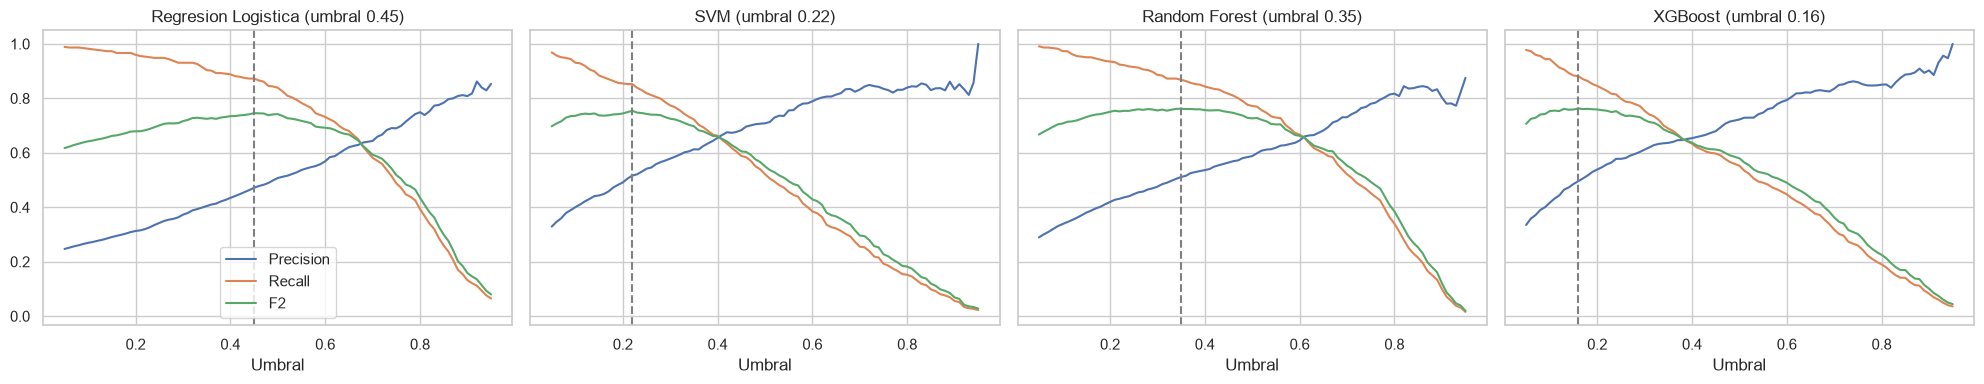
\includegraphics[width=0.95\textwidth]{figuras/umbrales.png}
\caption{Precisión, recall y $F_2$ según el umbral de decisión de cada modelo, con las predicciones fuera de muestra del conjunto de entrenamiento. La línea punteada marca el umbral elegido.}
\label{fig:umbrales}
\end{figure*}

Como los modelos base y los optimizados se evalúan con el mismo ROC AUC en validación cruzada, esa comparación es equivalente, mientras que las métricas dependientes del umbral de la Tabla~\ref{tab:defecto} (umbral 0.5) y de la Tabla~\ref{tab:optimizados} (umbral elegido) no deben compararse entre sí sin considerar el cambio de umbral.

Los modelos se ajustaron con todo el entrenamiento y se evaluaron una sola vez en el conjunto de prueba. Los cuatro detectan a casi los mismos hombres con deficiencia, 98 o 99 de los 112, con 13 o 14 casos que se escapan, por lo que la diferencia está en las falsas alarmas, 80 en el SVM y en el Random Forest, 97 en XGBoost y 118 en la Regresión Logística (Figura~\ref{fig:matrices}). El resultado coincide con la validación cruzada en que los tres modelos no lineales son casi equivalentes y la Regresión Logística queda detrás en precisión (0.454 contra más de 0.50). El umbral elegido es lo que hace útiles a los modelos, ya que con el umbral estándar de 0.5 el recall en la prueba cae de 0.884 a 0.509 en el SVM y a 0.473 en XGBoost, y a 0.705 en Random Forest y 0.795 en Regresión Logística, es decir, que dejarían escapar a entre el 20\% y el 53\% de los casos, aunque con menos falsas alarmas (por ejemplo 23 en lugar de 80 en el SVM).

La Tabla~\ref{tab:test} detalla el conteo de aciertos y errores en la prueba con el umbral elegido, y la Tabla~\ref{tab:umbral05} muestra lo que pasaría con el umbral estándar de 0.5, donde la precisión sube (por ejemplo a 0.712 en el SVM) pero el recall baja a 0.47 o 0.51 en XGBoost y SVM.

\begin{table}[t]
\centering
\footnotesize
\setlength{\tabcolsep}{3pt}
\caption{Evaluación en el conjunto de prueba con el umbral elegido (503 hombres, 112 con deficiencia).}
\label{tab:test}
\begin{tabular}{l c c c c c c c}
\toprule
Modelo & Exact. & F1 & AUC & TN & FP & FN & TP \\
\midrule
Reg. Logística & 0.738 & 0.598 & 0.866 & 273 & 118 & 14 & 98 \\
SVM (RBF) & 0.815 & 0.680 & 0.901 & 311 & 80 & 13 & 99 \\
Random Forest & 0.813 & 0.676 & 0.892 & 311 & 80 & 14 & 98 \\
XGBoost & 0.781 & 0.643 & 0.898 & 294 & 97 & 13 & 99 \\
\bottomrule
\end{tabular}
\end{table}

\begin{table}[t]
\centering
\footnotesize
\setlength{\tabcolsep}{3pt}
\caption{Evaluación en el conjunto de prueba con el umbral estándar de 0.5 (el ROC AUC no cambia).}
\label{tab:umbral05}
\begin{tabular}{l c c c c c c}
\toprule
Modelo & Exact. & Prec. & Recall & F1 & FP & FN \\
\midrule
Reg. Logística & 0.775 & 0.497 & 0.795 & 0.612 & 90 & 23 \\
SVM (RBF) & 0.845 & 0.712 & 0.509 & 0.594 & 23 & 55 \\
Random Forest & 0.831 & 0.603 & 0.705 & 0.650 & 52 & 33 \\
XGBoost & 0.833 & 0.679 & 0.473 & 0.558 & 25 & 59 \\
\bottomrule
\end{tabular}
\end{table}

\subsection{Comparación con el estado del arte}

La Tabla~\ref{tab:sota} compara este trabajo con cinco estudios que usan NHANES. Que el AUC de aquí sea mayor al de otros estudios no permite afirmar que los modelos sean mejores, y la diferencia debe interpretarse con las salvedades que siguen.

\begin{table*}[!t]
\centering
\footnotesize
\caption{Comparación con cinco estudios que usan NHANES. Las métricas son las reportadas por cada estudio y los protocolos no son equivalentes.}
\label{tab:sota}
\begin{tabular}{l p{4.2cm} p{4.2cm} c c}
\toprule
Autor / año & Modelo & Dataset (hombres) & Métrica & Resultado \\
\midrule
Yu et al., 2025 \cite{yu2025} & LightGBM (mejor) y SVM; también GBDT, CatBoost, RF y XGBoost & NHANES 2011 a 2014 (2628), 18 predictoras & AUC & 0.746 (LGBM); 0.713 (SVM) \\
Zhang et al., 2025 \cite{zhang2025} & Índice TyG-WHtR (mejor de nueve índices) & NHANES 2013 a 2016 (1514) & AUC & 0.776 \\
Guo et al., 2025 \cite{guo2025} & Índice TyG-WHtR (mejor de 15 índices) & NHANES 2011 a 2016 (3540) & AUC & 0.762 \\
Xu y Li, 2024 \cite{xu2024} & Índice cardiometabólico & NHANES 2013 a 2020 (5012) & AUC & 0.724 \\
Goulian et al., 2026 \cite{goulian2026} & Regresión logística (explicativa) & NHANES 2011 a 2016 y 2021 a 2023 (10357) & Razón de momios & 2.69 (obesidad); sin AUC \\
\midrule
Este trabajo & Reg. Logística, SVM, RF, XGBoost (13 predictoras, con hormonas) & NHANES 2021 a 2023 (2514), prueba de 503 & AUC & 0.866, 0.901, 0.892, 0.898 \\
\bottomrule
\end{tabular}
\end{table*}

\textbf{Modelos y variables.} Los índices de Zhang et al. \cite{zhang2025}, Guo et al. \cite{guo2025} y Xu y Li \cite{xu2024} son combinaciones simples de pocas medidas, mientras que Yu et al. \cite{yu2025} y este trabajo entrenan modelos con varias predictoras, y la principal diferencia es que aquí se usan SHBG, estradiol, LH y FSH, del mismo eje hormonal que la testosterona, mientras que los índices se calculan con medidas corporales y metabólicas más indirectas, lo que es probablemente la razón principal del AUC mayor frente a ellos. \textbf{Preprocesamiento y partición.} Yu et al. \cite{yu2025} usan una partición 80/20 con validación cruzada de 5 folds, igual que aquí, pero los estudios de índices son de naturaleza distinta, ya que evalúan indicadores calculados y no modelos entrenados, por lo que no aplica una partición equivalente. \textbf{Métricas y definición de clase.} El ROC AUC es la única métrica común, y como Yu et al. \cite{yu2025} reportan un recall de 1.000 en sus seis modelos no se puede comparar el recall ni la precisión. Además, los ciclos de NHANES, la prevalencia (de 20.3\% a 25.8\%) y el tamaño de la muestra cambian, y el conjunto de prueba de este trabajo tiene solo 112 casos positivos, lo que agrega incertidumbre a cualquier diferencia. Por todo eso, la comparación solo permite decir que el desempeño de este trabajo es del mismo orden o mayor que el reportado, y no que supere al estado del arte. Los estudios de Novaes et al. \cite{novaes2021} y Kivrak et al. \cite{kivrak2024} no usan NHANES y no se incluyen en la tabla, pero coinciden en que XGBoost es un buen clasificador base y en que el desbalance requiere cuidado.

\subsection{Análisis gráfico de resultados}

Las curvas ROC de la Figura~\ref{fig:roc} muestran que el SVM, el Random Forest y XGBoost casi se superponen y que la Regresión Logística queda por debajo en la zona de falsos positivos de 0.2 a 0.5, y los puntos marcan la operación de cada modelo con su umbral, a un recall cercano a 0.88 con tasas de falsos positivos de 0.20 a 0.30. Como la clase positiva es minoritaria, la Figura~\ref{fig:pr} muestra las curvas precisión-recall, donde el SVM obtiene el mayor promedio de precisión (0.726), seguido por XGBoost (0.699), Regresión Logística (0.682) y Random Forest (0.647), y el azar equivale a la prevalencia (0.223). Cabe notar que Random Forest, con un ROC AUC mayor que la Regresión Logística, tiene un AP menor, lo que se debe a que su precisión cae más en la zona de recall bajo, y que las curvas se cruzan, por lo que ningún modelo domina en todo el rango.

\begin{figure}[t]
\centering
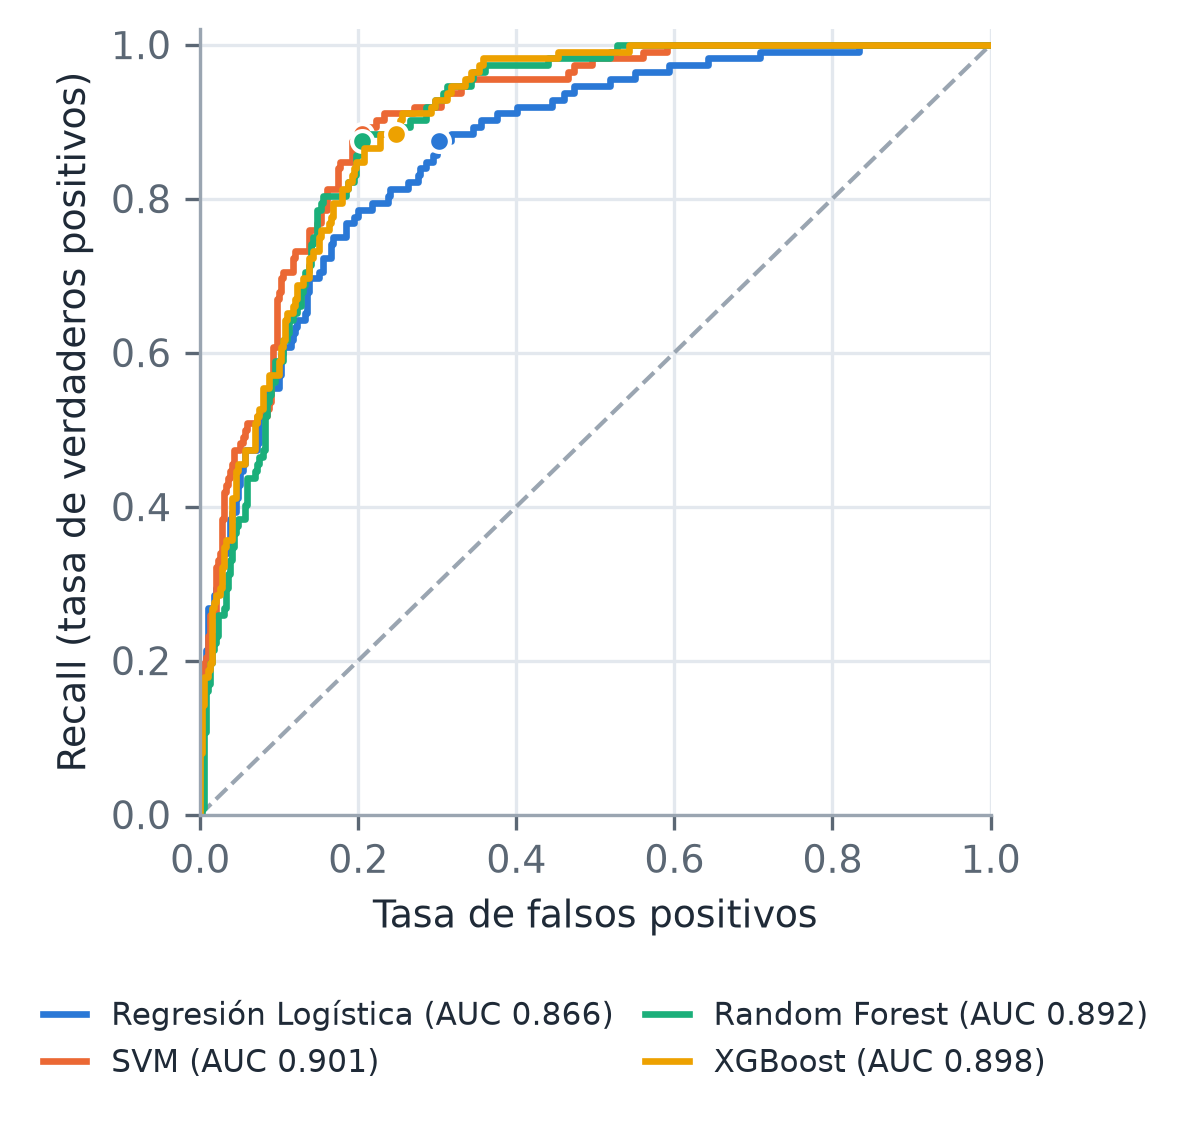
\includegraphics[width=0.88\columnwidth]{figuras/curvas_roc.png}
\caption{Curvas ROC en el conjunto de prueba. Los puntos marcan la operación de cada modelo con su umbral. La línea punteada es el azar.}
\label{fig:roc}
\end{figure}

\begin{figure}[t]
\centering
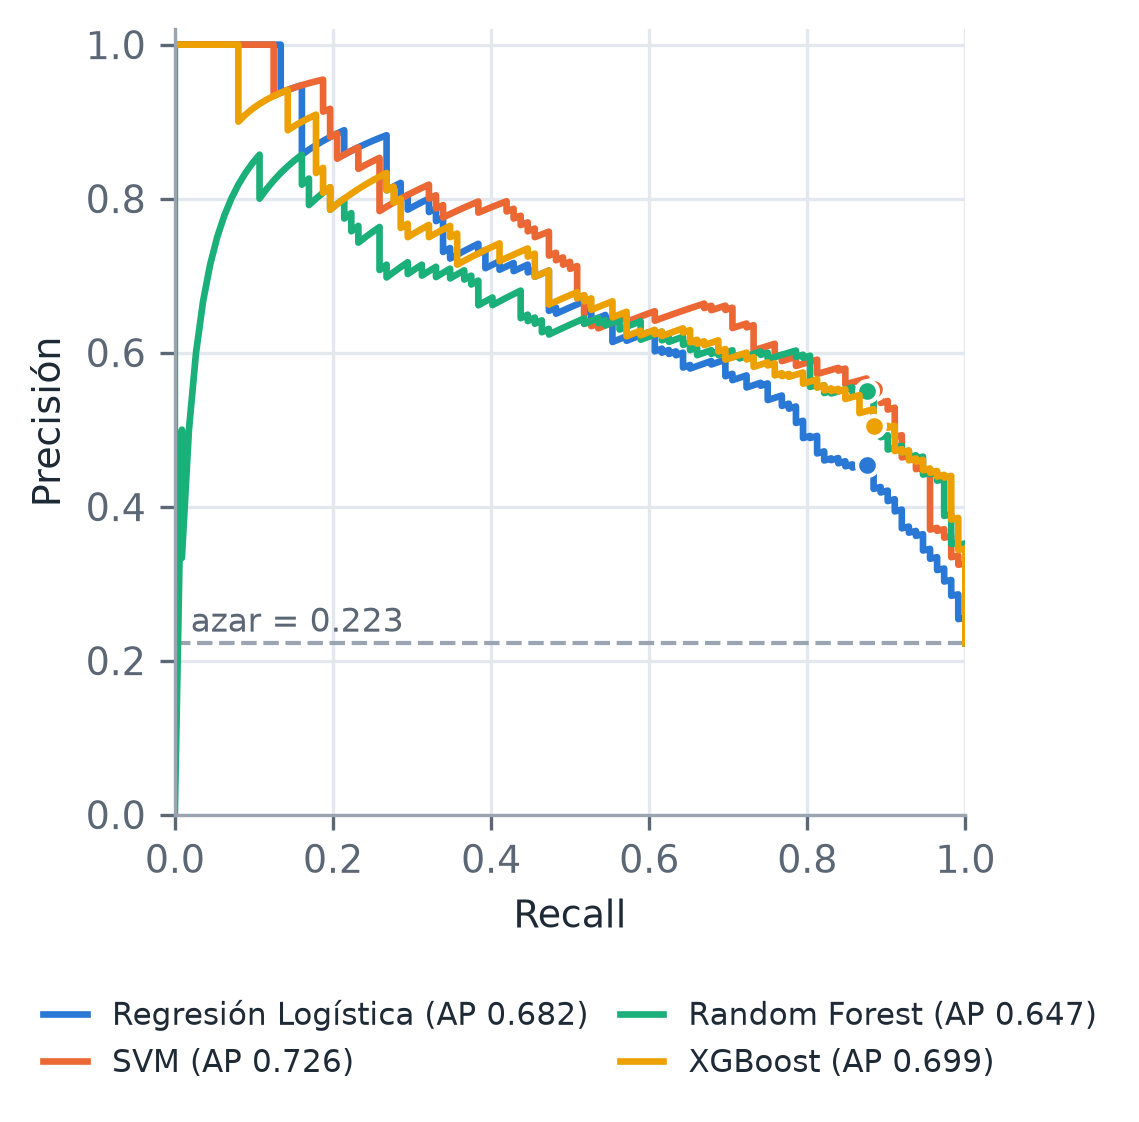
\includegraphics[width=0.88\columnwidth]{figuras/curvas_pr.png}
\caption{Curvas precisión-recall en el conjunto de prueba (AP: promedio de precisión). Los puntos marcan la operación de cada modelo con su umbral. La línea punteada es la prevalencia.}
\label{fig:pr}
\end{figure}

\begin{figure*}[!t]
\centering
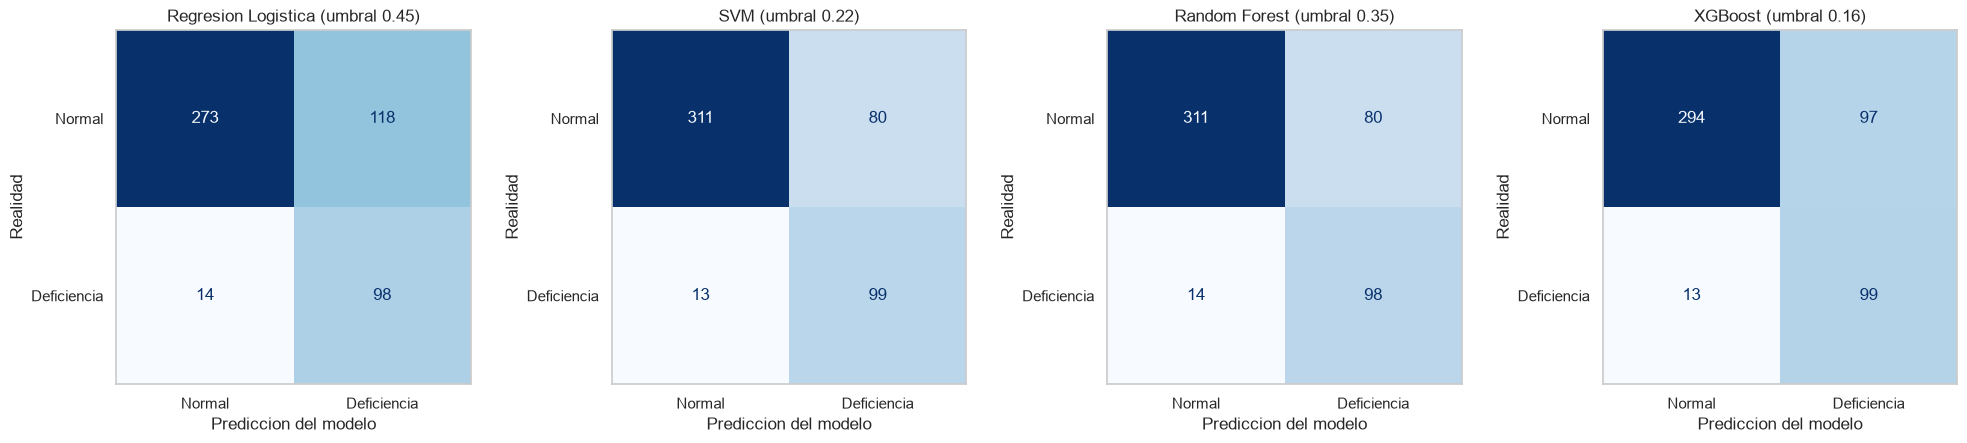
\includegraphics[width=0.95\textwidth]{figuras/matrices_confusion.png}
\caption{Matrices de confusión en el conjunto de prueba (503 hombres) con el umbral de cada modelo. Con el mismo recall, los modelos se distinguen por el número de falsos positivos.}
\label{fig:matrices}
\end{figure*}

Los tres tipos de modelo coinciden en las variables más importantes (Figura~\ref{fig:importancia}), SHBG y estradiol, que ocupan el primer y segundo lugar tanto en Random Forest (0.26 y 0.22) como en XGBoost (0.14 y 0.12) y que en la Regresión Logística tienen los coeficientes más grandes y negativos, lo que significa que a menor SHBG y menor estradiol, mayor probabilidad de deficiencia. Después aparecen la cintura, el IMC y la edad en los modelos de árboles, y en la Regresión Logística el IMC, la FSH y la edad tienen coeficientes positivos, mientras que la cintura casi no recibe coeficiente, seguramente porque se parece mucho al IMC (correlación de 0.92). La escolaridad y la raza aportan muy poco.

\begin{figure*}[!t]
\centering
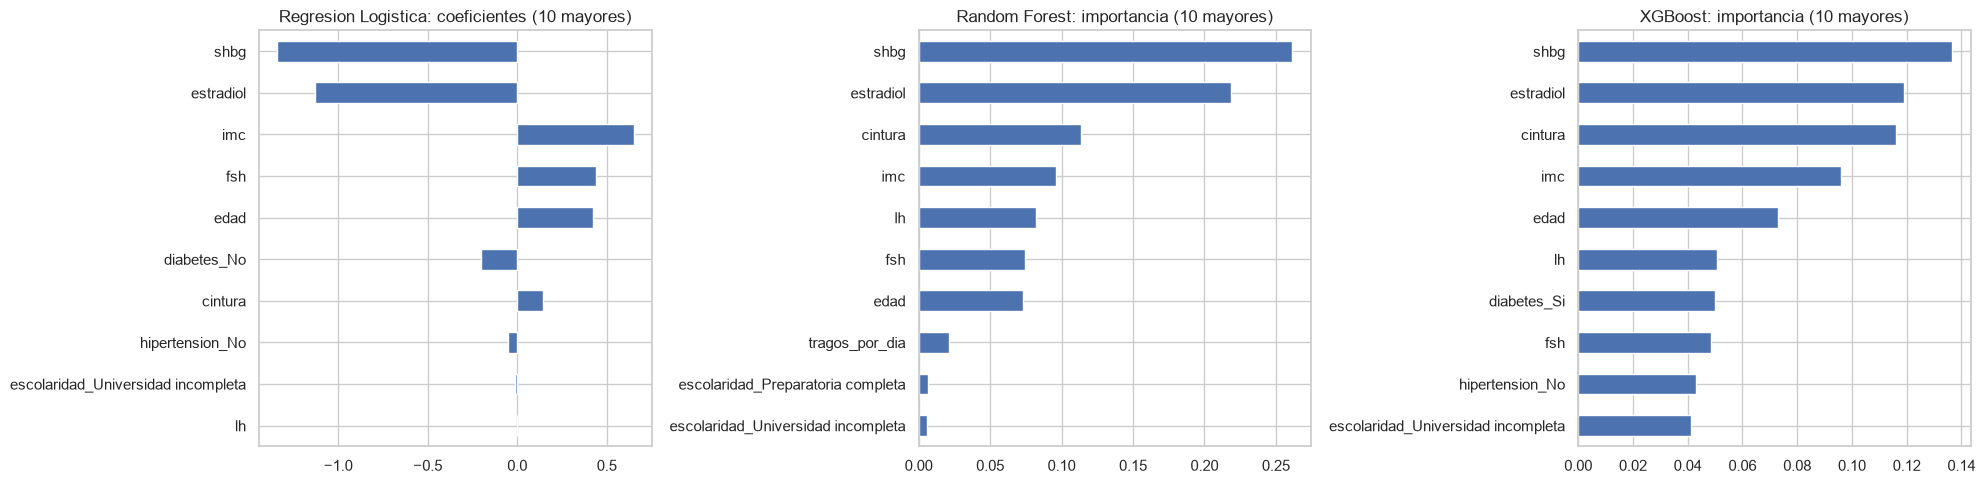
\includegraphics[width=0.95\textwidth]{figuras/importancia_variables.png}
\caption{Coeficientes de la Regresión Logística e importancia de variables de Random Forest y XGBoost (las 10 principales).}
\label{fig:importancia}
\end{figure*}

\subsection{Discusión de resultados}

\textbf{Mejor modelo.} El SVM obtuvo el mejor ROC AUC (0.901), el mejor $F_1$ (0.680) y el mejor AP (0.726) en la prueba, pero XGBoost y Random Forest quedaron a menos de 0.01 de ROC AUC, una diferencia menor que la desviación entre folds (0.008 a 0.022) y que la incertidumbre de un conjunto de prueba con 112 positivos, por lo que no puedo afirmar que uno sea claramente mejor que los otros dos. En validación cruzada el orden fue distinto (XGBoost 0.896, Random Forest 0.894, SVM 0.884), lo que confirma que se trata de un empate técnico. La Regresión Logística fue el modelo más débil, sobre todo en precisión, aunque es el más fácil de interpretar y su diferencia con los demás es de unos 0.03 de ROC AUC, lo que sugiere que la relación entre las variables y la deficiencia es principalmente suave y cercana a lo lineal.

\textbf{Base contra optimizado y características de los datos.} La optimización sirvió sobre todo para regularizar XGBoost y para compensar el desbalance con el umbral, y no tanto para subir el ROC AUC de los demás. Lo que pudo influir en los resultados es que SHBG y estradiol, que están fisiológicamente ligadas a la testosterona, concentran la importancia en los tres tipos de modelo, que la obesidad (cintura e IMC) y la diabetes aportan señal adicional, en línea con Goulian et al. \cite{goulian2026}, y que las clases están desbalanceadas, lo que hace que la precisión sea baja (45\% a 55\%) aun con un recall alto, es decir, que casi la mitad de las alertas son falsas alarmas.

\textbf{Comparabilidad, limitaciones y mejoras.} Los resultados son del mismo orden o mayores que los de la literatura con NHANES, pero la comparación está limitada por las diferencias de ciclo, variables y protocolo descritas en la sección anterior. Entre las limitaciones del experimento está la partición única, que con 112 positivos hace inconclusas las diferencias pequeñas, que los umbrales se eligieron con la prevalencia de este conjunto (en otra población la precisión sería distinta), que los modelos se entrenaron solo con el 80\% de los datos para conservar válida la prueba, y que las probabilidades no son un riesgo clínico calibrado. Como mejoras, se podría repetir la validación con varias particiones o con validación cruzada anidada, probar un ensamble de los modelos, validar con otro ciclo de NHANES o con otra población, y calibrar las probabilidades.

%==========================================================================
\section{Conclusiones}
\label{sec:conclusiones}

Se cumplió el objetivo de construir y comparar cuatro modelos de clasificación para la deficiencia de testosterona con un mismo protocolo sin fuga de información, y de ponerlos a disposición en una interfaz web. El SVM obtuvo el mejor resultado en el conjunto de prueba (ROC AUC de 0.901 y $F_1$ de 0.680), pero XGBoost (0.898) y Random Forest (0.892) quedaron dentro de la variación entre folds, por lo que el mejor modelo no se distingue claramente de los otros dos, y la Regresión Logística (0.866) fue la más débil en precisión (0.454 contra más de 0.50).

Entre los hallazgos, el umbral de decisión resultó tan importante como el modelo, ya que con 0.5 los modelos dejan escapar a entre el 20\% y el 53\% de los casos y con el umbral elegido detectan a cerca del 88\%, a cambio de que casi la mitad de las alertas sean falsas, y SHBG y estradiol fueron las variables más importantes en los tres tipos de modelo. Esto implica que las herramientas son aceptables como apoyo para decidir a quién pedirle un análisis de sangre entre hombres con síntomas o factores de riesgo, pero no como diagnóstico ni como tamizaje de la población general, que la guía de la Endocrine Society no recomienda \cite{bhasin2018}.

Como limitaciones, la partición es única, el conjunto de prueba tiene solo 112 casos positivos, la definición de la deficiencia usa una sola medición y los datos son de Estados Unidos, y como trabajo futuro se propone reentrenar con todos los datos, probar ensambles, validar con otro ciclo de NHANES o con datos de otra población y calibrar las probabilidades.

%==========================================================================
\bibliographystyle{IEEEtran}
\bibliography{referencias}

\end{document}
